\section{Illustrative Simulation}
\label{sec:sim}

Code and data to reproduce all simulations and figures in this paper are available at \url{https://anonymous.4open.science/r/cert_fore/}.

To confirm the kink condition (Corollary~\ref{cor:kink}) is not vacuous, we simulate the model under $f(c) = a\sqrt{c}$, $L(q) = b/(q+1)$, with $a = 0.30$, $b = 6.80$, $\beta = 0.95$, $\delta = 0.045$, $\tau = 0.80$, $p_H = 1.0$, $\rho = 0.30$ — chosen for tractability, not because the mechanism depends on them (Section~\ref{sec:sim-functionalform} confirms a structurally unrelated pair).

At $q=\tau$, $c^*(p_H)=0.0818$ and $c^*(p_L)=0.0084$, giving $f(c^*(p_H))=0.0858$ and $f(c^*(p_L))=0.0275$: the kink condition $f(c^*(p_L))<\delta\leq f(c^*(p_H))$ holds. Figure~\ref{fig:qc}(a) plots the resulting $q_t$ against a no-discount ablation ($p$ held at $p_H$ throughout). Starting from $q_0=0.30$, both trajectories climb identically while exposed; the foreclosure trajectory is first certified at $t=8$, peaks at $q=0.825$, and declines to $q=0.481$ by $t=39$ despite never failing a subsequent audit, while the ablation continues to $q=1.348$. Figure~\ref{fig:qc}(b) shows investment falling by an order of magnitude ($0.085\to0.008$) in the single period spanning certification, with no recovery.

\begin{figure}[t]
\centering
\begin{minipage}{0.49\linewidth}
\centering
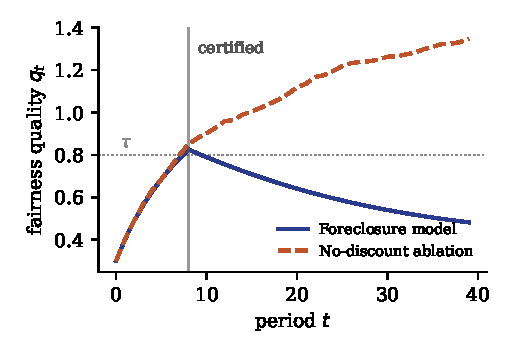
\includegraphics[width=\linewidth]{figures/fig_q.pdf}
\\ (a) Fairness quality $q_t$
\end{minipage}
\hfill
\begin{minipage}{0.49\linewidth}
\centering
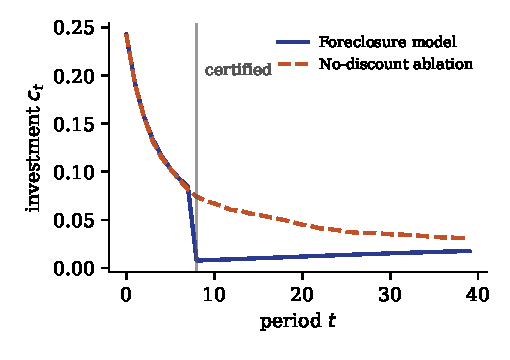
\includegraphics[width=\linewidth]{figures/fig_c.pdf}
\\ (b) Investment $c_t$
\end{minipage}
\caption{(a) The foreclosure model's quality trajectory peaks exactly at certification ($t=8$) and declines, while the no-discount ablation keeps improving under constant scrutiny. (b) Investment falls roughly tenfold in the single period spanning certification, with no recovery.}
\label{fig:qc}
\end{figure}

\subsection{Recurring Audits: Simulating Both Cases}
\label{sec:sim-recurring}

We verify Theorem~\ref{prop:recurring} on the same parameterization, using the closed form $q^*(p) = \sqrt{p\,\beta\,a^2 b / (2\delta)} - 1$ (Appendix~\ref{app:derivation}): $q^*(p_H)=1.542$. At $\rho=0.30$ ($q^*(p_L)=0.392<\tau<q^*(p_H)$: Case B), simulating~\eqref{eq:pt-recurring} for 120 periods produces sustained cycling: over $t\geq60$, $q_t$ oscillates between $0.783$ and $0.840$ with a period of 3--4 audit cycles, time-average $0.813$, strictly below $q^*(p_H)$. At $\rho=0.60$ ($\tau\leq q^*(p_L)=0.969$: Case A), the firm converges to a stable, permanently certified steady state near $q^*(p_L)$ — still strictly below $q^*(p_H)$, so the welfare loss persists even without cycling. Figure~\ref{fig:recurring} plots both.

\begin{figure}[t]
\centering
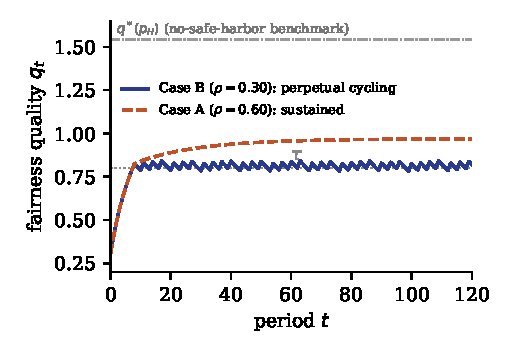
\includegraphics[width=0.55\linewidth]{figures/fig_recurring.pdf}
\caption{Recurring audits: at $\rho=0.30$ (Case B) the firm cycles indefinitely across $\tau$; at $\rho=0.60$ (Case A) it settles into permanent certification, below $q^*(p_H)$ in both cases.}
\label{fig:recurring}
\end{figure}

\subsection{Robustness Checks}
\label{sec:sim-robustness}

Four robustness checks; the $\rho$-sweep's extra figure and detail, and the real-disclosures calibration's full detail, are in Appendix~\ref{app:extra-sim}.

\paragraph{Safe-harbor discount.} Sweeping $\rho\in(0.05,0.95)$ at $\tau=0.80$ (Figure~\ref{fig:rhosweep}) confirms the Case A/B split is not a knife-edge artifact: the boundary falls at $\rho_A(\tau)=0.5015$, matching Proposition~\ref{prop:heterogeneous}'s cutoff to four decimals, with time-averaged quality in the cycling region staying flat in $[0.804,0.817]$ across a tenfold range of $\rho$ — once cycling, the outcome is insensitive to exactly how strong the discount is, only to whether it is strong enough to place the firm there. (This sweep also supplies the data behind Sections~\ref{sec:heterogeneous} and~\ref{sec:regulator}.) Separately sweeping $\beta\in[0.80,0.99]$ and $\delta\in[0.010,0.090]$ confirms cycling is robust to $\beta$ and that $\delta$ moves the firm through all three regimes, consistent with Corollary~\ref{cor:deltacompstat}.

\begin{figure}[t]
\centering
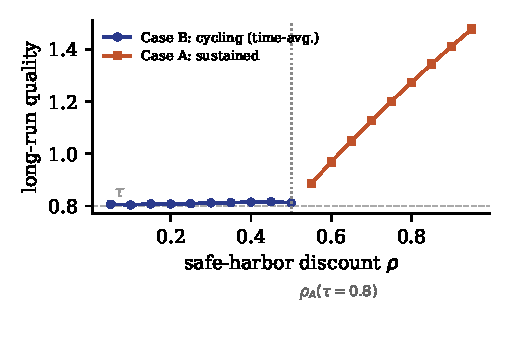
\includegraphics[width=0.55\linewidth]{figures/fig_rhosweep.pdf}
\caption{Long-run quality as $\rho$ varies, $\tau=0.80$ fixed. The Case A/B boundary at $\rho_A=0.5015$ matches the closed-form prediction; within Case B, the time-average is roughly flat across a wide range of $\rho$.}
\label{fig:rhosweep}
\end{figure}

\paragraph{Functional form.}\label{sec:sim-functionalform} The results above use $f(c)=a\sqrt{c}$, $L(q)=b/(q+1)$. To check this is not load-bearing, we repeat the four central checks under a structurally different pair, $f(c)=ac^{1/3}$ and $L(q)=be^{-q}$ ($a=0.55$, $b=3.20$), recalibrating $\tau=3.80$ to sit between this pair's own steady states ($q^*(p_L)=3.218$, $q^*(p_H)=4.422$ at $\rho=0.30$) rather than reuse the original calibration's scale. Table~\ref{tab:functionalform} shows all four reproduce. (One subtlety: $c^*(p)$ and $\delta$ are not directly commensurate, so the kink condition is stated via $f(c^*(p))$ rather than $c^*(p)$ itself — the two comparisons coincide numerically under $\sqrt{c}$ because $f$ is near-linear there, but diverge visibly here.)

\begin{table}[t]
\centering
\footnotesize
\caption{Central results reproduced under $f(c)=a\,c^{1/3}$, $L(q)=b\,e^{-q}$ ($a=0.55$, $b=3.20$, $\tau=3.80$, $\rho=0.30$).}
\label{tab:functionalform}
\begin{tabular}{@{}p{0.32\linewidth}p{0.6\linewidth}@{}}
\toprule
Check & Result \\
\midrule
Discrete investment collapse & $c^*(p_L)=0.0002 < c^*(p_H)=0.0014$ \\[2pt]
Kink condition & $f(c^*(p_L))=0.034 < \delta=0.045 \leq f(c^*(p_H))=0.061$ \\[2pt]
Single-certification kink & peaks at $t{=}55$ ($q{=}3.815$), declines to $q{=}3.221$ by $t{=}300$ \\[2pt]
Recurring-audit cycling & $123$ regime switches in tail; mean $3.803 < q^*(p_H){=}4.422$ \\
\bottomrule
\end{tabular}
\end{table}

\paragraph{Firm heterogeneity.}\label{sec:sim-heterogeneous} Evaluating Corollary~\ref{cor:aggwelfare} under $\rho_i\sim\mathrm{Uniform}(0.05,0.95)$ gives aggregate welfare $0.983$, a $36.2\%$ loss relative to $q^*(p_H)$ with $50.2\%$ of firms cycling; under $\rho_i\sim\mathrm{Beta}(4,2)$ (weighted toward weak safe-harbor effects, a conservative stand-in for a population where severe effects are the exception), loss falls to $30.4\%$ with $18.9\%$ cycling but does not disappear — even Case (a) firms sustain quality strictly below $q^*(p_H)$ whenever $\rho_i<1$ (Table~\ref{tab:aggwelfare}).

\begin{table}[t]
\centering
\caption{Aggregate welfare loss under two firm-population distributions, $\tau=0.80$, $q^*(p_H)=1.542$.}
\label{tab:aggwelfare}
\begin{tabular}{@{}lccc@{}}
\toprule
Distribution of $\rho_i$ & $W_{\mathrm{agg}}$ & Loss (\% of $q^*(p_H)$) & \% cycling \\
\midrule
Uniform$(0.05,0.95)$ & $0.983$ & $36.2\%$ & $50.2\%$ \\
Beta$(4,2)$, rescaled & $1.072$ & $30.4\%$ & $18.9\%$ \\
\bottomrule
\end{tabular}
\end{table}

\paragraph{Calibrating to real audit disclosures.}\label{sec:calibration} NYC Local Law 144 disclosure data grounds $\tau=0.80$ empirically. Wright et al.~\cite{wright2024null} found 96\% of 386 impact-ratio measurements (late 2023) exceeded $0.8$; Gerchick et al.~\cite{gerchick2025auditing}, through November 2024, found a larger below-threshold share (23--28\% of group-level results) — a discrepancy we attribute to sampling and methodology differences rather than resolve. The latter is inconsistent with a population of only Case A firms (which, once certified, stay at or above $\tau$) and more consistent with Case B firms cycling around it, though we stop short of testing the dynamic predictions directly: only 13 same-employer report-pairs are documented, with overwritten disclosures and no tool-version identifiers (Appendix~\ref{app:extra-sim}, Section~\ref{sec:discussion}).

\subsection{Imperfect Observation}
\label{sec:sim-imperfectobs}

We verify Proposition~\ref{prop:imperfectobs} using the logistic $\pi(q)=1/(1+\exp(-(q-\tau)/\sigma))$, with investment evaluated against scrutiny at the firm's \emph{current} state $p(q_t)$, exactly as specified.\footnote{An earlier version instead evaluated scrutiny at the post-investment state and added a term not implied by the proposition; it is kept in the replication code for reference only and is not the source of the numbers here.} The unique fixed point $q^{**}(\sigma)$ matches the closed-form prediction, converging to $\tau=0.800$ as $\sigma\to0$ for every $\sigma$ down to $10^{-5}$. The simulated \emph{trajectory}, however, only converges above $\sigma_0\approx0.0063$ (where the fixed point's slope crosses $-1$); below it, it settles into persistent bounded oscillation instead (Figure~\ref{fig:imperfectobs}). Just above threshold, $q^{**}(0.01)=0.809$; at $\sigma=1.0$, $q^{**}=0.995$, below $q^*(p_H)=1.542$ but well above $\tau$ and the hard-threshold cycling mean $0.8125$. Below threshold, amplitude widens as $\sigma\to0$ and the time-average converges to $0.812$, matching that cycling mean to three decimals.

\begin{figure}[t]
\centering
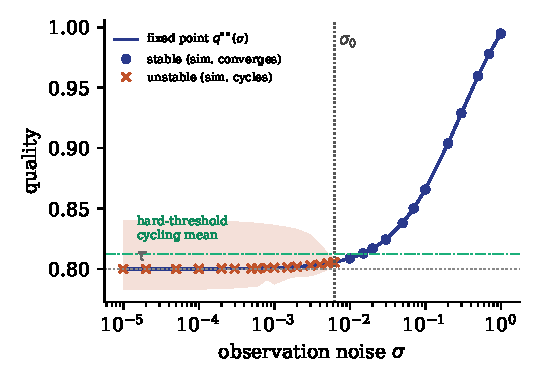
\includegraphics[width=0.55\linewidth]{figures/fig_imperfectobs.pdf}
\caption{Quality under imperfect observation as detection noise $\sigma$ varies (log scale). The fixed point $q^{**}(\sigma)$ converges to $\tau$ as $\sigma\to0$ regardless of stability; circles mark simulated convergence, crosses mark cycling (shaded: tail range) below $\sigma_0$.}
\label{fig:imperfectobs}
\end{figure}

Above $\sigma_0$, higher noise raising quality is the opposite of the naive ``noisier audits are worse'' intuition; Section~\ref{sec:imperfectobs} explains why this does not generalize to noise that is merely uninformative rather than cliff-edge-removing.
